\section{Checking Property Preservation}
\label{sec:lts-transformation:proppres}

In this section, we show how property preservation of transformations can be checked by generating networks from rule systems and comparing the LTSs of these networks.
Figure~\ref{fig:lts-transformation:check-generation} gives an overview of the approach.

\begin{figure}[hbt]
\centering
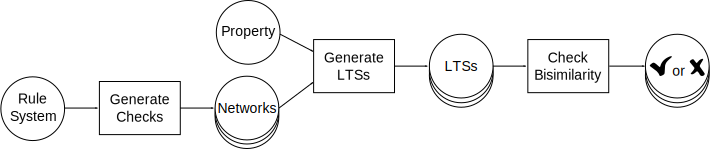
\includegraphics[scale=0.6]{lts-transformation/figs/check-generation}
\caption{Checking property preservation by comparing LTSs}
\label{fig:lts-transformation:check-generation}
\end{figure}

First, networks are generated based on the left and right-hand sides of transformation rules.
Then, the network LTSs corresponding to these networks are generated, while applying maximal hiding regarding the property at hand.
Finally, property preservation is checked by comparing the network LTSs generated from left-hand sides of transformation rules with the network LTSs of the corresponding right-hand sides.
If all pairs of LTSs are divergence-sensitive branching bisimilar, the rule system preserves the property at hand.

More formally, a terminating, confluent rule system $\Sigma$ is $\Sf$-preserving for a property~$\Sf \in \dsbrLmu$ iff $\models_{\smodel} \Sf \iff \models_{T_{\Sigma} (\smodel)} \Sf$ for all networks~$\smodel$.
Thus, if $\Sigma$ is $\Sf$-preserving and $\models_{\smodel} \Sf$, we can conclude that~$\models_{T_{\Sigma} (\smodel)} \Sf$ without rechecking property~$\Sf$ for network~$T_{\Sigma} (\smodel)$.
Since $\dsbrLmu$ is compatible with maximal hiding and DSBB, as discussed in Section~\ref{subsec:lts-transformation:lmu}, $\Sigma$ is $\Sf$-preserving if $\maxabstr(\smodel) \dsbbis \maxabstr(T_{\Sigma} (\smodel))$.
In this section, we discuss under which conditions a rule system implies the bisimilarity of $\maxabstr(\smodel)$ and $\maxabstr(T_{\Sigma} (\smodel))$.
The most important condition roughly boils down to checking whether, after some appropriate rewriting, the left and right patterns of the transformation rules are divergence-sensitive branching bisimilar after maximal hiding.
If this is the case, then applying the rules does not result in a network with structurally different behavior.

Without loss of generality, for each network~$\smodel = \networktuple$ and rule system~$\Sigma = \rulesystemtuple$, we assume that each $r \in R$ has exactly one match to some $\Pi[i]$ and that each $\Pi[i]$ is matched on by exactly one $r$.
This is expressed by indexing the~$r \in R$ such that rule~$r_i$ is matched on~$\Pi[i]$.
If~$R$ contains only one rule, we omit its index.
Since~$\Sigma$ is confluent, the results of this section can be lifted to the more general case where rules may have an arbitrary number of matches.
With this assumption, it can also safely be assumed that all the $\actions{i}$ are disjoint.
If this is not the case, some renaming of actions and a corresponding modification of the synchronization rules can resolve this.

\subsection{Extended Transformation Rules}
To show that a rule system~$\Sigma$ preserves a property~$\Sf$ for every network~\smodel, we show that a divergence-sensitive branching bisimulation between the states of~$\maxabstr(\smodel)$ and~$\maxabstr(T_{\Sigma} (\smodel))$ can be constructed based on the divergence-sensitive branching bisimulations between networks constructed from the transformation rules.
To construct these networks from the transformation rules, we extend the transformation rules with self-loops on the glue-states.
The matches of the glue-states of a given transformation rule may be part of transitions that are not present in the patterns of this rule.
The transformation rules are extended to make explicit that such transitions may exist.
Each self-loop is labeled with an action uniquely related to the corresponding state.

\begin{definition}
\label{def:lts-transformation:extendedtransformationrule}
Given an LTS transformation rule $r = \transruletuple{r}$, the corresponding extended transformation rule is defined as~$r_\kappa = \langle \Llts^r_\kappa, \Rlts^r_\kappa \rangle$, where
\begin{itemize}
\item
$\Llts^r_\kappa = \langle \states{\Llts^r}, \actions{\Llts^r} \cup \{ \kappa_s \mid s \in \states{\Llts^r} \cap \states{\Rlts^r} \}, \transitions{\Llts^r} \cup \{ \langle s, \kappa_s, s \rangle \mid s \in \states{\Llts^r} \cap \states{\Rlts^r} \}, \initialstates{\Llts^r} \rangle$;
\item
$\Rlts^r_\kappa = \langle \states{\Rlts^r}, \actions{\Rlts^r} \cup \{ \kappa_s \mid s \in \states{\Llts^r} \cap \states{\Rlts^r} \}, \transitions{\Rlts^r} \cup \{ \langle s, \kappa_s, s \rangle \mid s \in \states{\Llts^r} \cap \states{\Rlts^r} \}, \initialstates{\Rlts^r} \rangle$.
\end{itemize}
\end{definition}

\noindent
We assume that the $\kappa$-actions are not originally in $\actions{\Llts^r}$.
Without these loops, a DSBB check of patterns could consider two deadlock states to be bisimilar, while they are actually different glue-states that are possibly matched on states with different outgoing transitions not present in the patterns.
For example, without the dashed $\kappa$-loops, states~$\it{ii}$ and~$\it{iii}$ in Figure~\ref{fig:lts-transformation:kappa} would be related if~$a,b \in h_{\actions{}}(\Sf)$.
With the $\kappa$-loops, however, they are not related, as indicated by the cross.
Thus, the extra transitions ensure that $\Llts^r_\kappa \dsbbis \Rlts^r_\kappa$ iff there exists a divergence-sensitive branching bisimulation that relates all the glue-states to themselves.
A glue-state $s$ in $\Llts^r_\kappa$ (or $\Rlts^r_\kappa$) with self-loop $s\ \smash{\xrightarrow{\kappa_s}}\ s$ must at least be related to itself in $\Rlts^r_\kappa$ (or $\Llts^r_\kappa$) since it is the only state where a $\kappa_s$-transition is enabled.

\begin{figure}[hbt]
\centering
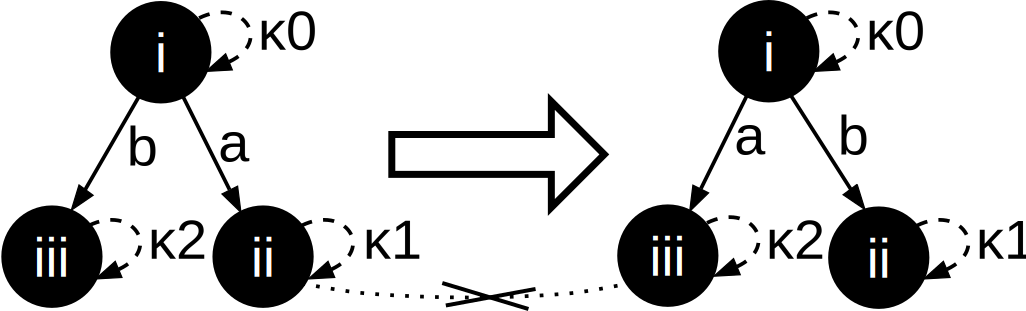
\includegraphics[scale=0.2]{lts-transformation/figs/kappa-loops}
\caption{An extended transformation rule}
\label{fig:lts-transformation:kappa}
\end{figure}

\subsection{Synchronizing Behavior}
If a rule system consists of multiple transformation rules, then multiple LTS transformations can be applied in a single transformation step.
To check $\Sf$-preservation of such rule systems, we need to take possible synchronization between different rule patterns into~account.

\begin{figure}[hbt]
\centering
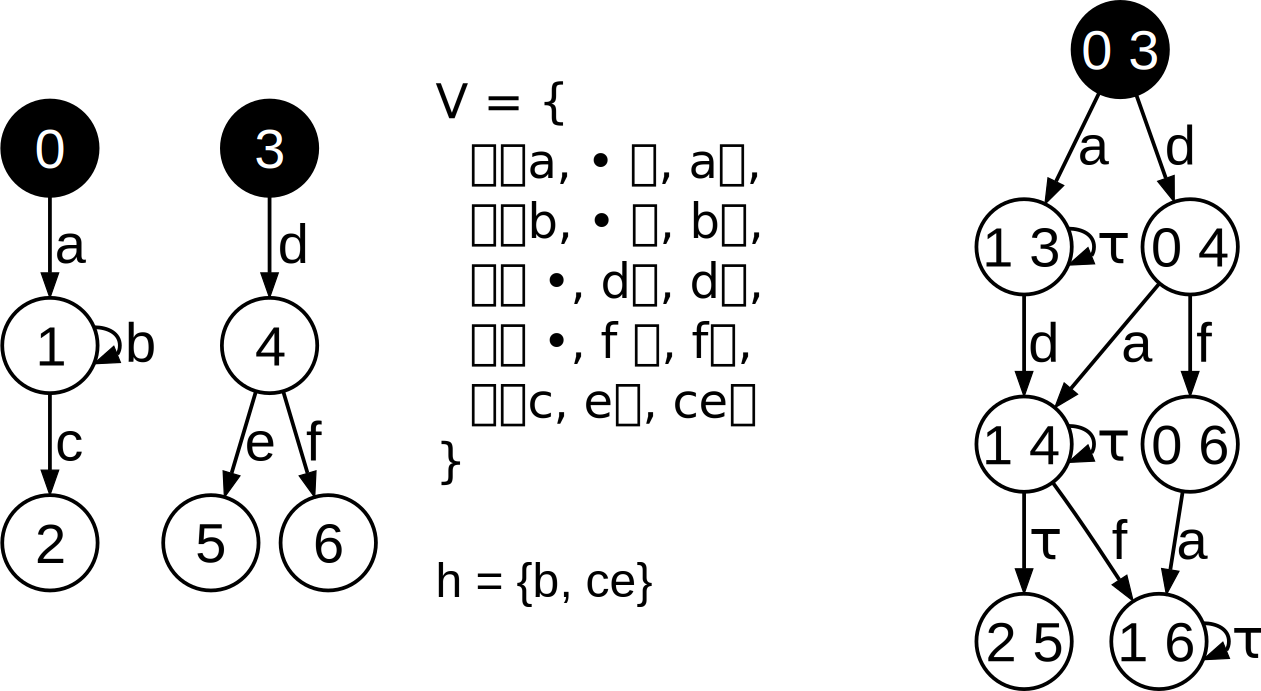
\includegraphics[scale=0.2]{lts-transformation/figs/comparison-network}
\caption{A network and the corresponding network LTS}
\label{fig:lts-transformation:comparison-network}
\end{figure}

In Figure~\ref{fig:lts-transformation:comparison-network}, a network involving synchronization and the corresponding network LTS are shown.
The network LTS is obtained after hiding the actions in~$h$, shown in the middle of the figure, which is the hiding set for some property~$\Sf$.
The rule system shown on the left of Figure~\ref{fig:lts-transformation:preserving-rules} can be applied to the network of Figure~\ref{fig:lts-transformation:comparison-network}.
Individually, the rules seem to fundamentally change the behavior of the process LTSs, as shown in the middle of Figure~\ref{fig:lts-transformation:preserving-rules}.
However, since the rule system also adds the new synchronization rules~$\langle\langle c1, e1 \rangle, c1e1\rangle$ and~$\langle\langle c2, \bullet \rangle, c2\rangle$, and the actions~$\it{c1e1}$ and~$\it{c2}$ can be hidden,
the final network LTS, as shown on the right of the figure, is bisimilar to the one before transformation.
To incorporate such possible dependencies between rule patterns, we developed a $\Sf$-preservation check involving networks of rule patterns.

\begin{figure}[hbt]
\centering
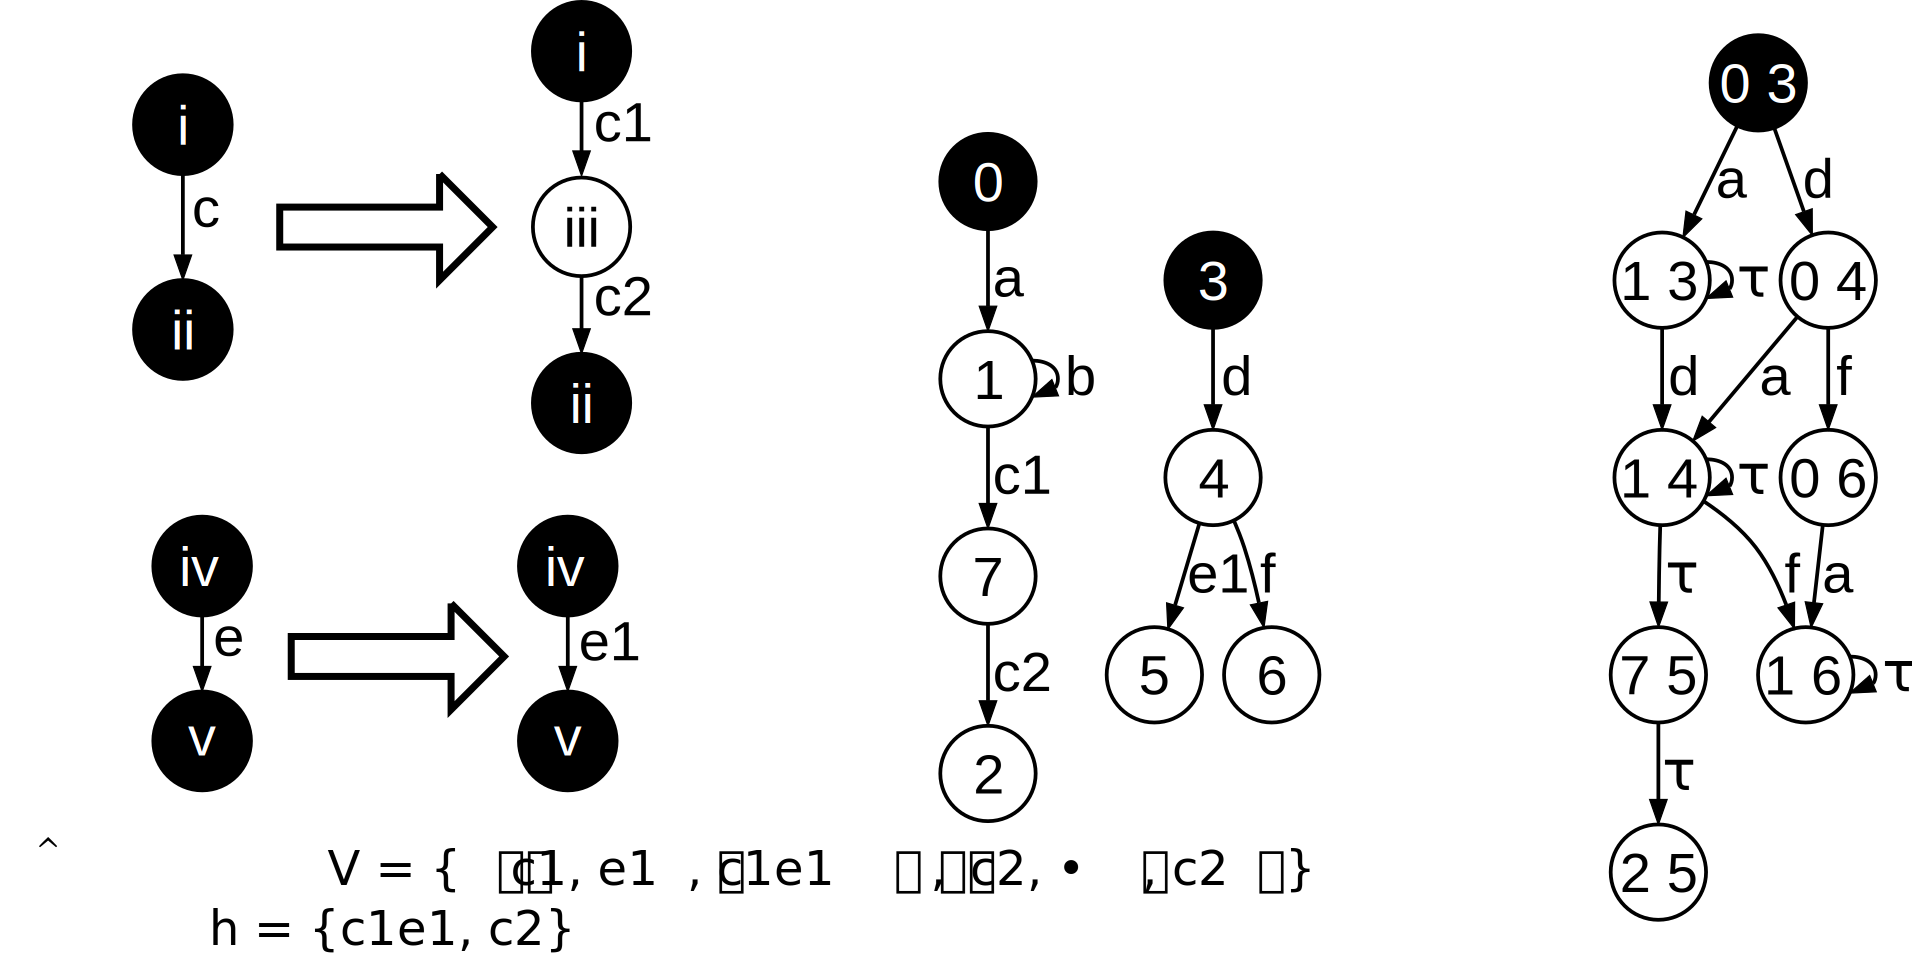
\includegraphics[scale=0.2]{lts-transformation/figs/preserving-rules}
\caption{A rule system and an example of its application}
\label{fig:lts-transformation:preserving-rules}
\end{figure}

In general, when considering transformation rules that affect synchronizing actions and thus involve multiple process LTSs, it cannot be determined whether a given rule system~$\Sigma = \rulesystemtuple$ involving such rules is $\Sf$-preserving by just analyzing the $\Llts^\ri$ and $\Rlts^\ri$ of all $\ri \in R$.
However, this can be done if $\Sigma$ has a number of properties regarding synchronizing behavior of a network $\smodel$, which we together call synchronization uniformity.

Before we can give a definition of synchronization uniformity, we need a number of auxiliary definitions.
The set of actions involved in synchronization vector~$\vectornot{t}$ is ${\actions{}}(\vectornot{t}) = \{ a \mid \exists i \in 1..n. \vectornot{t}[i] = a \wedge a \neq \bullet \}$,
and the set of actions involved in synchronization rules in~\synchrules with multiple processes is $\syncactions (\synchrules) = \{a \mid \exists \langle \vectornot{t},a' \rangle \in \synchrules. a \in {\actions{}}(\vectornot{t}) \wedge |{\it Ac}(\vectornot{t})|>1 \}$.
The set of indices of process LTSs that can potentially synchronize with behavior in $\Llts^\ri$ according to a synchronization rule in \synchrules is $\inv(\Llts^\ri, \synchrules) = \bigcup \{ {\it Ac}(\vectornot{t}) \mid \syncruletuple \in \synchrules \wedge \vectornot{t}[i] \in \actions{\Llts^\ri} \}$.
This definition states that $j$ is in $\inv(\Llts^\ri, \synchrules)$ iff there exists a synchronization rule $\syncruletuple$ in $\synchrules$ such that both $i \neq \bullet$ and $j \neq \bullet$, i.e.\ both $i$ and $j$ are active for that rule, and the behavior in $\Pi[i]$ is matched on by transformation rule $\ri = \transruletuple{r_i}$.
The set of actions of process $j$ on which the actions in~$\Llts^\ri$ depend according to the synchronization rules in~\synchrules is $\dep^{\Llts^\ri}(j, \synchrules) = \{ \vectornot{t}[j] \mid \syncruletuple \in \synchrules \wedge \vectornot{t}[i] \in \actions{\Llts^\ri} \wedge \vectornot{t}[j] \neq \bullet \}$.
In other words, the set of all actions $\bigcup_{t \in F} \{\vectornot{t}[j] \} \setminus \{\bullet\}$ constitutes $\dep^{\Llts^\ri}(j, \synchrules)$, where~$F$ represents the set of all synchronization rules applicable on $\Llts^\ri$.
Sets $\inv(\Rlts^\ri, \synchrules)$ and $\dep^{\Rlts^\ri}(j, \synchrules)$ are defined similarly.
Now, synchronization uniformity can be defined.

\begin{definition}
\label{def:lts-transformation:uniformity}
We say that rule system~$\Sigma = \rulesystemtuple$ is synchronization uniform w.r.t.\ network~$\smodel = \networktuple$ iff the following holds.
\begin{enumerate}
\item
$\forall a \in \actions{s} (\synchrules). (\exists \ri \in R. a \in \actions{\Llts^\ri}) \implies \forall s_1\xrightarrow{a}_{i} s_2 . s_1, s_2 \in m_\ri(\states{\Llts^\ri})$;
\item
$\forall \ri \in R, j \in \inv(\Llts^\ri, \synchrules). \dep^{\Llts^\ri}(j, \synchrules) \subseteq \actions{\Llts^\rj}$;
\item
$\forall \langle\vectornot{t},a\rangle \in \hat\synchrules, i \in 1..n. \vectornot{t}[i] = \bullet \vee \vectornot{t}[i] \in \actions{\Rlts^\ri}$.
\end{enumerate}
\end{definition}

The first condition states that if a transformation rule is applicable to a synchronizing transition, then it is applicable to all synchronizing transitions with the same label in~\smodel.
If this is not guaranteed, it becomes very hard to reason about the model after transformation because it is difficult to determine a priori exactly which transitions in different process LTSs will be able to synchronize in the network.
Therefore, predicting the effect of rewriting, for example, $a$-transitions in some places while keeping other $a$-transitions the same is as difficult.
Checking this condition requires inspecting the process LTSs of a network, unless we impose an additional restriction on rule systems.
If we require that all left-hand patterns of rules that modify synchronizing transitions consist of a single transition, the first condition holds, regardless of the structure of the process LTSs of~\smodel.
The second condition states that all actions that can synchronize with $\Llts^\ri$ are also transformed by $\Sigma$.
If this does not hold, it becomes hard to analyze the synchronizing behavior as appearing in transformation patterns.
In such cases, some of the behavior that is relevant for this analysis is not present in any of the patterns, which makes analysis based only on the rule system impossible.
Finally, the third condition states that each new synchronization rule~$\langle\vectornot{t},a\rangle \in \hat\synchrules$ involves actions from the $\Rlts^\ri$ of the corresponding rule~$\ri$ only.
It is crucial to rule out the possibility of transforming merely by introducing synchronization rules, because this also prevents analysis solely based on rule systems.
For example, if we define a new synchronization rule involving existing actions~$a$ and~$b$, and these actions were previously not allowed to synchronize, then we clearly change the model without actually transforming anything.

In the remainder of this chapter, we only consider rule systems that are synchronization uniform regarding a given model.
This may seem a big assumption, but in practice, one tends to transform synchronizing behavior in a uniform way.
Usually, synchronizing actions, say~$a$ and~$b$, represent communication.
If one wants to transform this behavior, it is natural to do this consistently in all places where~$a$ and~$b$ occur, and to transform the behavior of both communicating parties to keep them compatible with each other.

\subsection{Networks of transformation rules}

From a rule system, networks of transformation rules can be constructed.

\begin{definition}
\label{def:lts-transformation:rule-network}
For a model~$\smodel = \networktuple$, rule system~$\Sigma = \rulesystemtuple$, and a rule~$\ri \in R$, the vector~$\xi^\ri$ of transformation rules relevant for the behavior in $\Llts^\ri$ is defined as follows, for all $j \in 1..n$.

\[
\xi^\ri[j] =
\left\{
\begin{array}{ll}
\ast \mapsto \ast & {\rm if} ~ j \not\in \inv(\Llts^\ri, \synchrules) \\
r_{j,\kappa}	  & {\rm if} ~ j \in \inv(\Llts^\ri, \synchrules),
\end{array}
\right.
\]
\end{definition}

\noindent
where $\ast$ is a dummy state.
For a given vector $\xi^\ri$, $\xi_{\Llts}^\ri$ is the vector of left patterns of the extended transformation rules in~$\xi^\ri$, and $\xi_{\Rlts}^\ri$ is the vector of right patterns.
The networks~$\Xi_\Llts^\ri = (\xi_\Llts^\ri, \synchrules)$ and $\Xi_\Rlts^\ri = (\xi_\Rlts^\ri, \synchrules \cup \hat\synchrules)$ allow comparing synchronizing behavior in rule patterns, before and after transformation according to $\Sigma$, in particular involving~$\ri$.

\begin{figure}[hbt]
\centering
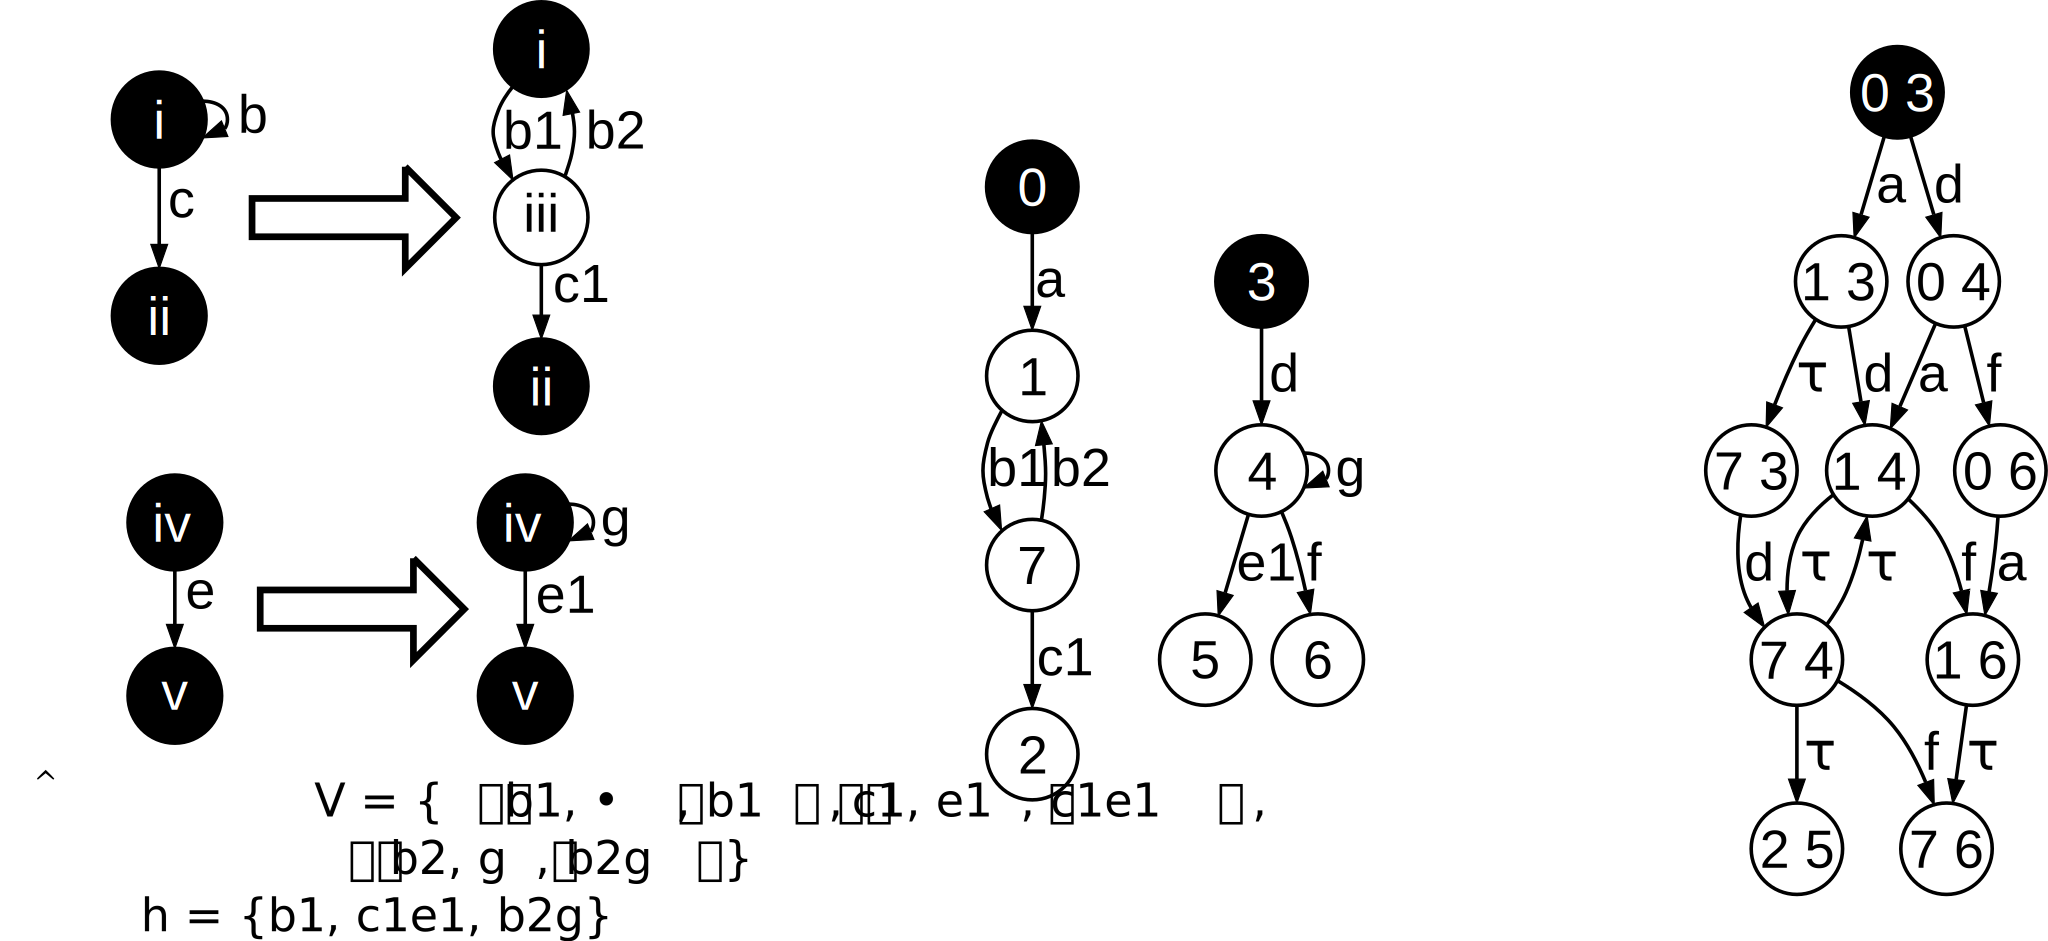
\includegraphics[scale=0.2]{lts-transformation/figs/non-preserving-rules}
\caption{A non-preserving transformation and an example of its application}
\label{fig:lts-transformation:non-preserving-trafo}
\end{figure}

On the left of Figure~\ref{fig:lts-transformation:non-preserving-trafo}, another example of a rule system is shown.
In general, this rule system is not $\Sf$-preserving.
Applying this rule system to the network in Figure~\ref{fig:lts-transformation:comparison-network} results in the network shown in the middle of Figure~\ref{fig:lts-transformation:non-preserving-trafo}.
The corresponding network LTS shown on the right of this figure is obtained after hiding the actions in~$h$.
The networks of the left and right patterns of the two transformation rules in this figure are shown in Figure~\ref{fig:lts-transformation:subsets-ltss:middle}.
Actions in~$h$ are hidden.
The dotted lines in this figure illustrate that a divergence-sensitive branching bisimulation exists for these two networks.

%%%\begin{figure}[hbt]
%%%\centering
%%%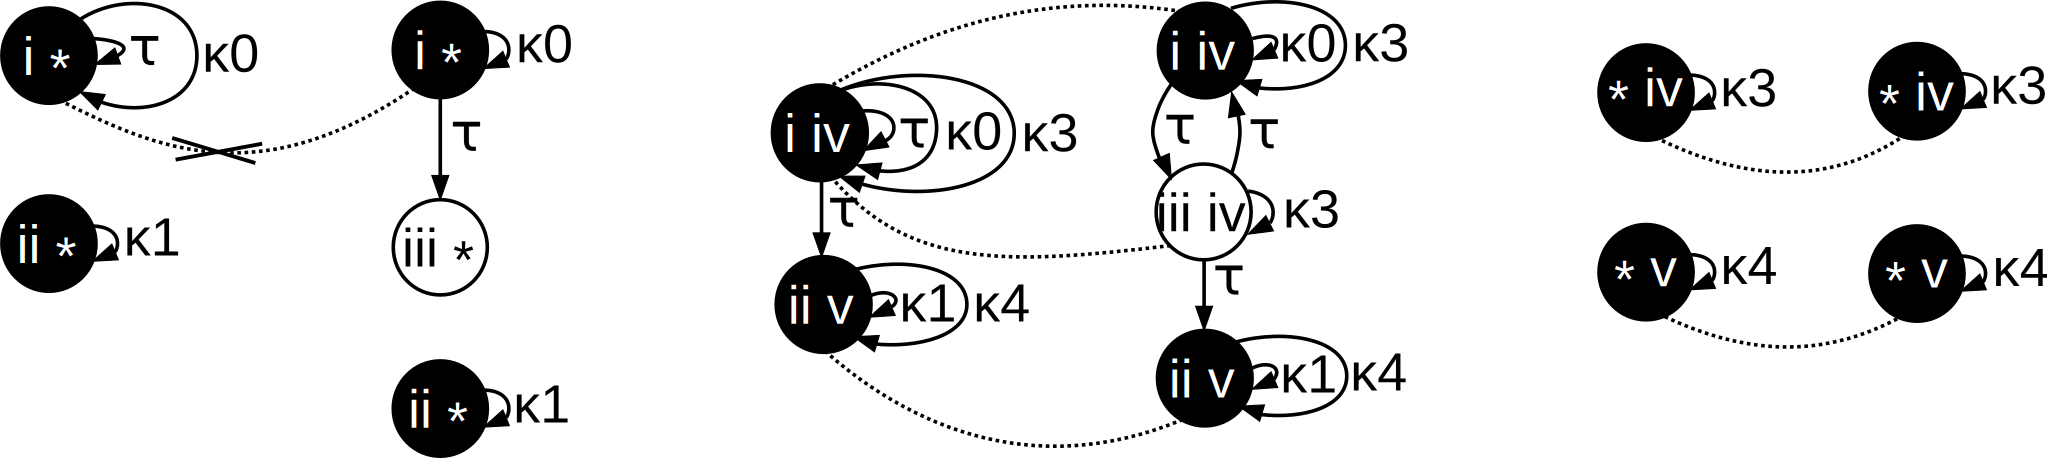
\includegraphics[scale=0.2]{lts-transformation/figs/subsets-ltss}
%%%\caption{Network LTSs of networks of transformation rules}
%%%\label{fig:lts-transformation:subsets-ltss}
%%%\end{figure}

\begin{figure}[hbt]
  \hfill
  \begin{subfigure}[b]{102pt}
    \centering
    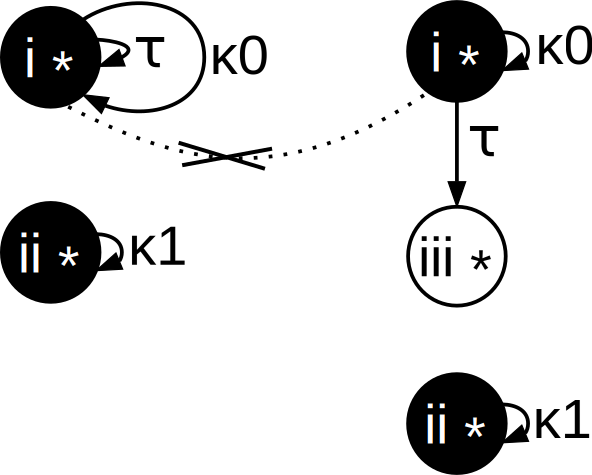
\includegraphics[scale=0.2]{lts-transformation/figs/subsets-ltss-left}
    \caption{}
    \label{fig:lts-transformation:subsets-ltss:left}
  \end{subfigure}
  \hfill
  \begin{subfigure}[b]{106pt}
    \centering
    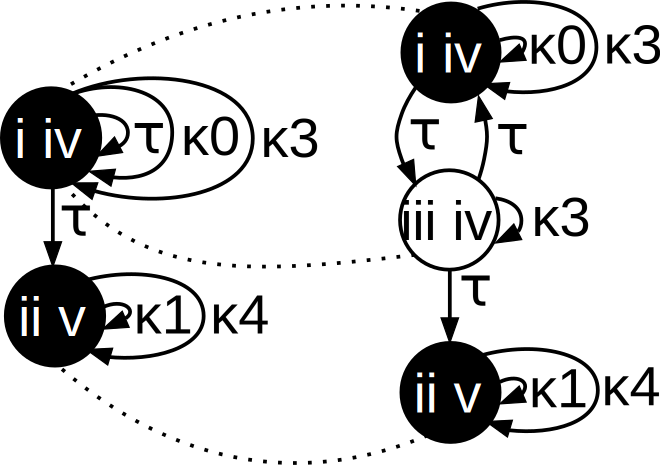
\includegraphics[scale=0.2]{lts-transformation/figs/subsets-ltss-middle}
    \caption{}
    \label{fig:lts-transformation:subsets-ltss:middle}
  \end{subfigure}
  \hfill
  \begin{subfigure}[b]{102pt}
    \centering
    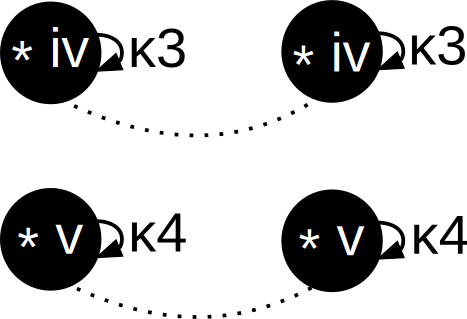
\includegraphics[scale=0.2]{lts-transformation/figs/subsets-ltss-right}
    \caption{}
    \label{fig:lts-transformation:subsets-ltss:right}
  \end{subfigure}
  \hfill
  \caption{Network LTSs of networks of transformation rules}
\end{figure}

Even though a divergence-sensitive branching bisimulation exists between the networks of the left and right patterns of the transformation rules in Figure~\ref{fig:lts-transformation:non-preserving-trafo}, the rule system is not \Sf-preserving.
This clearly shows that it is not sufficient to only take successful synchronization in account.
Instead, we also need to consider situations in which some parties are able to perform a synchronizing action whereas at least one other party involved in the synchronization is not.
For example, the state labeled (1 3) in Figure~\ref{fig:lts-transformation:comparison-network} has a $\tau$-loop that cannot be simulated by the network LTS in Figure~\ref{fig:lts-transformation:non-preserving-trafo}.
This $\tau$-loop is the result of hiding the $b$-loop of the leftmost process of Figure~\ref{fig:lts-transformation:comparison-network}.
This process can perform action~$b$ independently.
After transformation, however, a $\tau$-cycle can only result from interaction between the transformed process LTSs shown in the middle of Figure~\ref{fig:lts-transformation:non-preserving-trafo}.
In situations where both processes are able to interact successfully, an infinite number of $\tau$-actions can be performed, as shown in Figure~\ref{fig:lts-transformation:subsets-ltss:middle}.
However, if the required synchronization between processes is impossible, as is the case in the state labeled (1 3) in Figure~\ref{fig:lts-transformation:non-preserving-trafo}, only one $\tau$-action can be performed.

To be able to consider such scenarios, we define a projection operator on networks of transformation rules.

\begin{definition}
\label{def:lts-transformation:projection}
For each vector of transformation rules~$\xi^\ri$ and~$j \in 1..n$, the projection operator $/I$ ($I \subseteq 1..n$) is defined as follows.
\[
\xi^\ri/I[j] = \left\{
\begin{array}{ll}
\xi^\ri[j]                    & {\rm if} ~ j \in I \\
\ast \mapsto \ast & {\rm otherwise}
\end{array}
\right.
\]
\end{definition}

\noindent
This operator can similarly be applied on the vectors of patterns~$\xi_{\Llts}^\ri$ and~$\xi_{\Rlts}^\ri$, and we say that $\Xi_\Llts^\ri/I = (\xi_\Llts^\ri/I, \synchrules)$ and $\Xi_\Rlts^\ri/I = (\xi_\Rlts^\ri/I, \synchrules \cup \hat\synchrules)$, for a given model~$\smodel = \networktuple$ and rule system~$\Sigma = \rulesystemtuple$ such that $\ri \in R$.

Figure~\ref{fig:lts-transformation:subsets-ltss:left} shows the left and right patterns of the rule network that contains only the topmost transformation rule of Figure~\ref{fig:lts-transformation:non-preserving-trafo}.
The left pattern of this rule network is constructed from the left pattern of this transformation rule, using the synchronization rules and the hiding set of Figure~\ref{fig:lts-transformation:comparison-network}.
The right pattern of this rule network is constructed from the right pattern of this transformation rule, using the synchronization rules and the hiding set of Figure~\ref{fig:lts-transformation:non-preserving-trafo}.
Because these patterns are not divergence-sensitive branching bisimilar, as indicated by the cross, this rule system is not \Sf-preserving.
The remaining patterns are shown in Figure~\ref{fig:lts-transformation:subsets-ltss:right}.

\subsection{Constructing a Bisimulation Relation}
The following theorem formalizes our $\Sf$-preservation check.

\begin{theorem}
\label{theo:lts-transformation:checkpreservation}
Let $\smodel = \networktuple$ be a model and $\Sf \in \dsbrLmu$ a temporal property such that $\models_{\smodel} \Sf$.
Then $\Sigma = \rulesystemtuple$ is $\Sf$-preserving if the following holds, for all $\ri \in R$, $I \subseteq \inv(\Llts^\ri, \synchrules)$.
\begin{equation}
\maxabstr(\Xi_{\Llts}^\ri/I ) \dsbbis \maxabstr(\Xi_{\Rlts}^\ri/I )
\label{eq:lts-transformation:maintheo}
\end{equation}
\end{theorem}

Proving this theorem for a rule system~$\Sigma$ and a property~\Sf entails constructing a relation between~$\maxabstr(\smodel)$ and~$\maxabstr(T_{\Sigma} (\smodel))$ based on the divergence-sensitive branching bisimulations in equation~\ref{eq:lts-transformation:maintheo}, for some model~\smodel, and proving that this relation is a divergence-sensitive branching bisimulation too.
To describe the construction of this relation, we need a number of auxiliary definitions.

First, a state in the network LTS of network~\smodel is a vector $\vectornot{s} = \langle \vectornot{s}[1],\ldots, \vectornot{s}[n] \rangle$.
An arbitrary $\vectornot{s} \in \states{\smodel}$ can have up to $n$ elements that are matched on by some transformation rule.
For an LTS~$\graph$ and a transformation rule~$r = \transruletuple{r}$,
matching $m_r$ is extended to sets of states such that $m_r(\states{\Llts^r}) \subseteq \states{\graph}$ refers to the set of states to which the states in $\states{\Llts^r}$ are matched,
and $\hat m_r(\states{\Llts^r}) = \{ s \in m_r(\states{\Llts^r}) \mid m_r^{-1}(s) \not\in \states{\Rlts^r} \}$ refers to the states in~\states{\graph} that relate to non-glue-states in $\Llts^r$.
By definition, the latter states are those that are removed from~\graph by rule~$r$.
We denote the set of indices of elements in $\vectornot{s}$ matched on by the corresponding rule with $M(\vectornot{s}) = \{ i \mid \vectornot{s}[i] \in m_\ri(\states{\Llts^\ri}) \}$.
%%%%%%%%%%%%%%%%%%%%%%%%%%%%%%%%%%%%%%%
%%%%%%%%%%%%%%%%%%%%%%%%%%%%%%%%%%%%%%%
%%%%%%%%%%%%%%%%%%%%%%%%%%%%%%%%%%%%%%%
%In a similar way, $\hat M(\vectornot{s}) = \{ i \mid \vectornot{s}[i] \in \hat m_\ri(\states{\Llts^\ri}) \}$.
%%%%%%%%%%%%%%%%%%%%%%%%%%%%%%%%%%%%%%%
%%%%%%%%%%%%%%%%%%%%%%%%%%%%%%%%%%%%%%%
%%%%%%%%%%%%%%%%%%%%%%%%%%%%%%%%%%%%%%%
As indicated above, we assume that if $\vectornot{s}[i]$ is matched on, then it is matched on by rule $r_i$.
Furthermore, for a rule system~$\Sigma = \rulesystemtuple$ and a network~\smodel, a simulation relation exists between the states in~\smodel and those in the rule networks~$\Xi_\Llts^\ri/I$ as well as between the states in~$T_{\Sigma} (\smodel)$ and those in~$\Xi_\Rlts^\ri/I$.
This can be formalized as follows.
For a state vector $\vectornot{s}^*$ in a rule network~$\Xi_\Llts^{\ri}/I$ and a state vector $\vectornot{s}$ in an LTS network~$\smodel$, we say that $\vectornot{s}$ simulates $\vectornot{s}^*$, denoted $\vectornot{s}^* \vdash \vectornot{s}$, iff $\forall i \in 1..n. \vectornot{s}^*[i] \neq \ast \implies \vectornot{s}[i] = m_\ri(\vectornot{s}^*[i])$.
In other words, besides the $\ast$-states, all process states in $\vectornot{s}^*$ are matched on the corresponding states in $\vectornot{s}$.
Now, first of all, if $\vectornot{s}^* \vdash \vectornot{s}$, and $\vectornot{s}^*\xrightarrow{a} \vectornot{s}^*'$, then also $\vectornot{s}\xrightarrow{a} \vectornot{s}'$ and $\vectornot{s}^*' \vdash \vectornot{s}'$.
Second of all, in cases that $\vectornot{s}\xrightarrow{a} \vectornot{s}'$ and some synchronization vector~$\vectornot{t}$ enables transition~$\vectornot{s}\xrightarrow{a} \vectornot{s}'$, with ${\it Ac}(\vectornot{t}) \subseteq I$, ${\it Ac}(\vectornot{t}) \subseteq M(\vectornot{s})$, and ${\it Ac}(\vectornot{t}) \subseteq M(\vectornot{s}')$, then the involved behavior of every active $\Pi[i]$ ($i \in {\it Ac}(\vectornot{t})$) is matched on by $\ri$.
The definition for~$\Xi_\Rlts^{\ri}/I$ and~$T_{\Sigma} (\smodel)$ is similar.
These simulation relations are preserved after maximal hiding.

\begin{figure}[hbt]
\centering
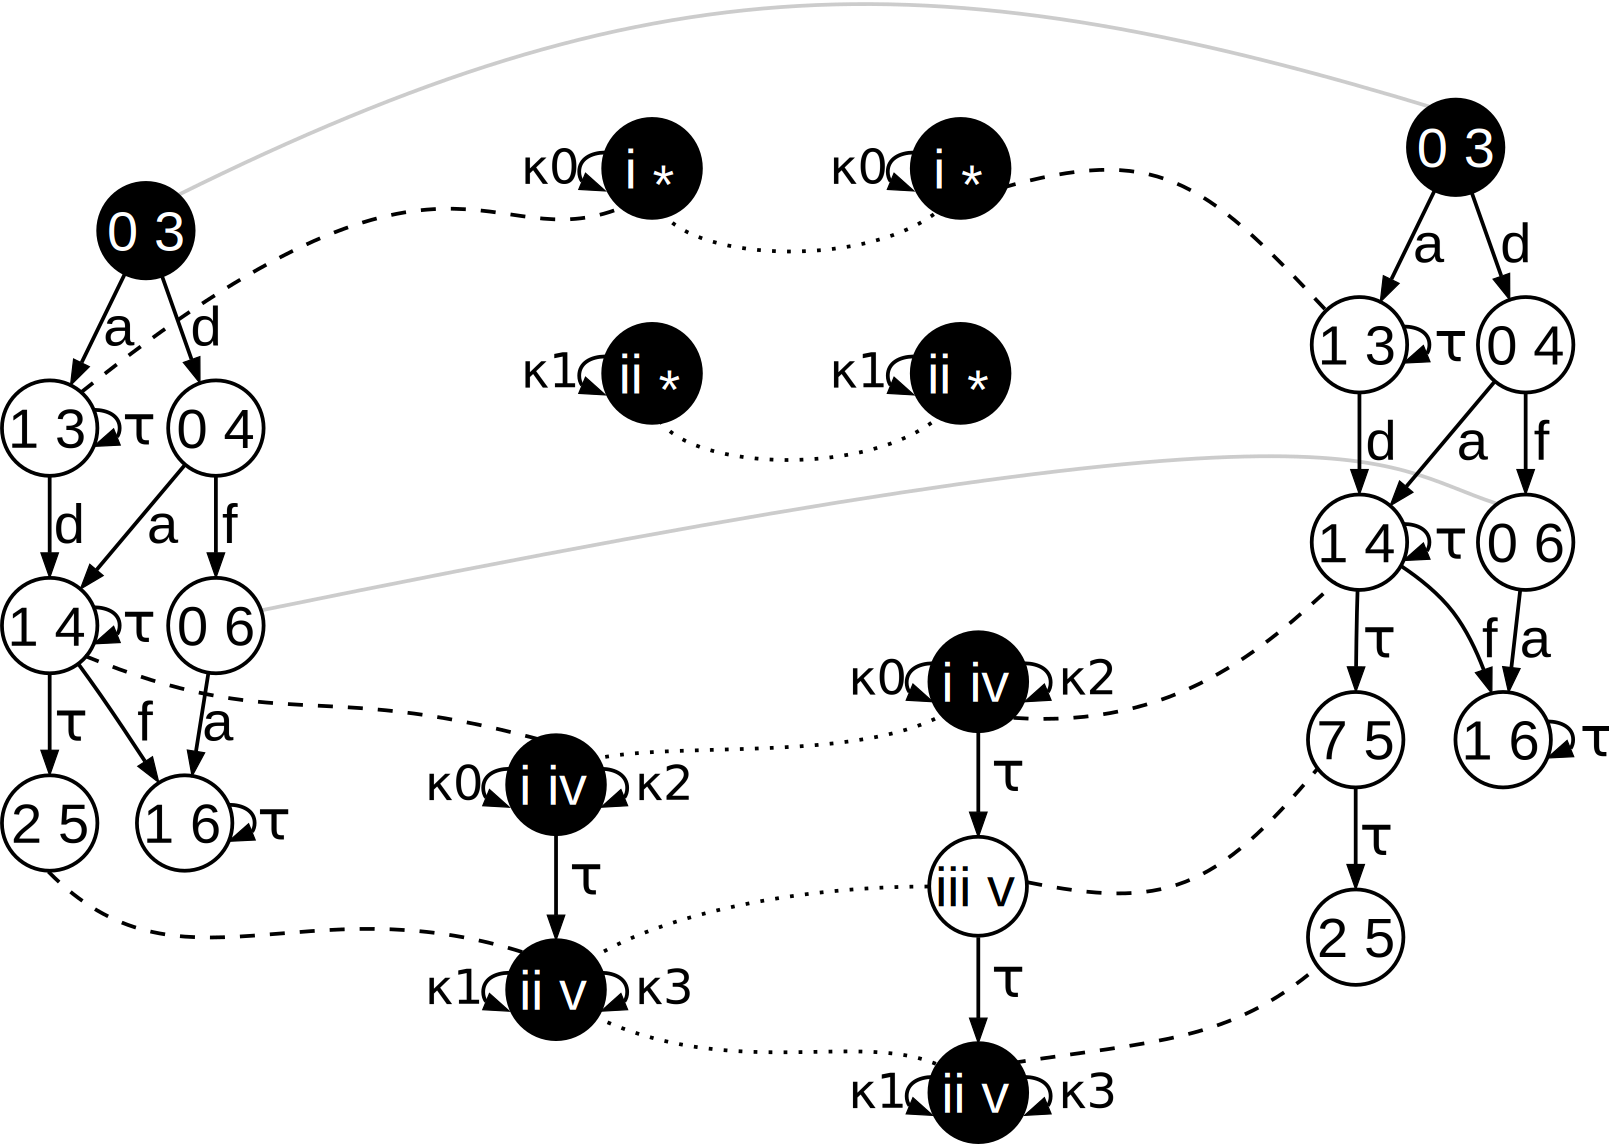
\includegraphics[scale=0.2]{lts-transformation/figs/relations}
\caption{Constructing a divergence-sensitive branching bisimulation}
\label{fig:lts-transformation:relations}
\end{figure}

A relation between two networks representing a model before and after transformation can be constructed by combining the bisimulations between pairs of rule networks with the simulation relations between model networks and rule networks.
In Figure~\ref{fig:lts-transformation:relations}, the dashed lines connect some of the states in the LTSs of the rule networks with the states in the LTSs of the models that simulate them.
The dotted lines in the figure denote the divergence-sensitive branching bisimulations between pairs of rule networks.
By combining these relations, states in the LTS on the left of the figure are related to states in the LTS on the right.
We refer to the relation formed by combining these relations as~$D$.
To increase the readability of the figure, not all states that are related according to~$D$ are connected.
For states~$\vectornot{s}$ of~$\smodel$ and~$\vectornot{p}$ of~$T_{\Sigma} (\smodel)$, we define $\vectornot{s}\ D'\ \vectornot{p}$ iff $\forall i \not \in M(\vectornot{s}) . \vectornot{s}[i] = \vectornot{p}[i]$.
In words, $D'$ relates all state vectors with exactly the same elements apart from those matched on by a transformation rule.
In a sense, $D'$ is a strong bisimulation for the behavior not subjected to transformation.
As mentioned above, not all states that are related according to~$D$ are connected in the figure.
Only those states of the LTS on the left of the figure are connected to states of the LTS on the right that are also related according to~$D'$.
Thus, the dashed and dotted lines together illustrate the relation~$(D \cap D')$ by connecting some of the states that are related according to this relation.
Relation~$D'' = \{ (\vectornot{s}, \vectornot{s}) \mid M(\vectornot{s}) = \emptyset \}$ relates all states that are not subjected to transformation.
The grey lines in Figure~\ref{fig:lts-transformation:relations} connect the states that are related according to~$D''$.
Given these relations, a relation~$C = (D \cap D') \cup D''$ can be constructed, which relates~$\maxabstr(\smodel)$ and~$\maxabstr(T_{\Sigma} (\smodel))$.
By considering the cases of Definition~\ref{def:lts-transformation:dsbbsim}, it can be shown that this relation is a divergence-sensitive branching bisimulation~\cite{EngelenWijsPropPres2012}. 